\documentclass[border=10pt]{standalone}
\usepackage{tikz}
\usetikzlibrary{positioning, shapes.geometric, arrows.meta, backgrounds, fit}

% Define colors (converting hex to RGB)
\definecolor{colorBook}{RGB}{225,245,255}
\definecolor{colorGrammar}{RGB}{255,244,225}
\definecolor{colorDict}{RGB}{255,244,225}
\definecolor{colorRLConvert}{RGB}{240,225,255}
\definecolor{colorSynthetic}{RGB}{240,225,255}
\definecolor{colorGym}{RGB}{225,255,225}
\definecolor{colorRewards}{RGB}{225,255,225}
\definecolor{colorCurriculum}{RGB}{225,255,225}
\definecolor{colorModel}{RGB}{255,225,225}

\begin{document}
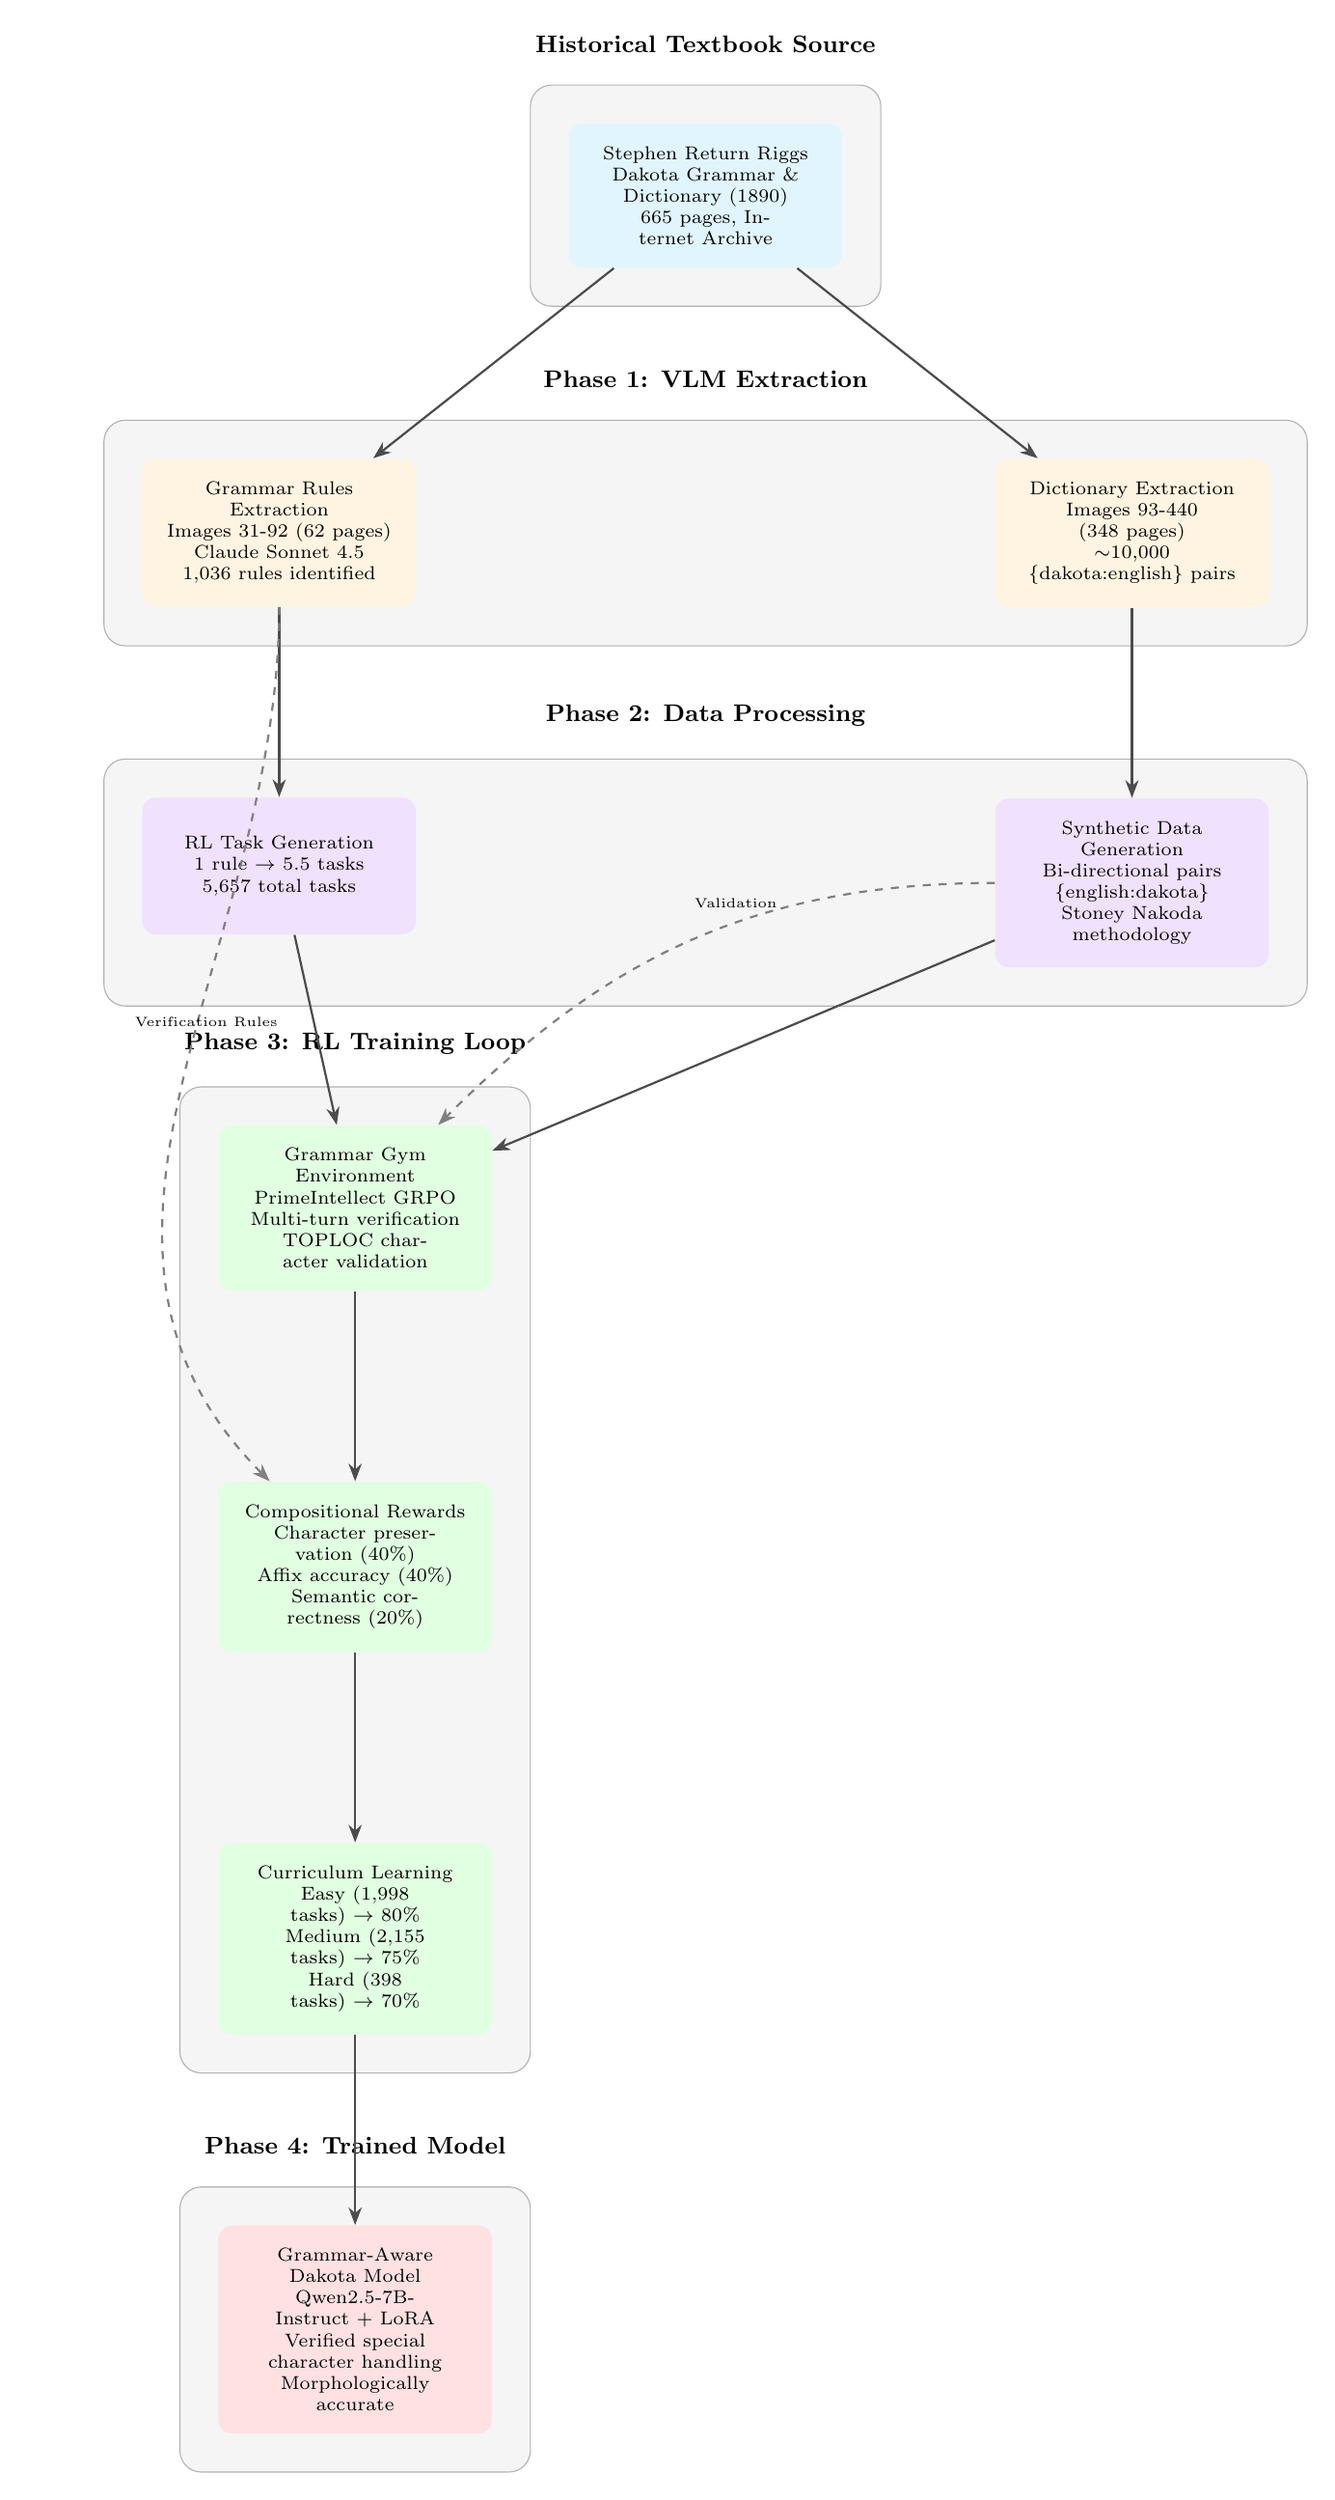
\begin{tikzpicture}[
    node distance=1.8cm,
    box/.style={rectangle, rounded corners=5pt, minimum width=3.2cm, minimum height=1.8cm, 
                text width=3cm, align=center, font=\scriptsize, inner sep=0.3cm},
    arrow/.style={->, >=Stealth, thick, color=black!70},
    dasharrow/.style={->, >=Stealth, dashed, thick, color=black!50}
]

% Source subgraph nodes
\node[box, fill=colorBook] (Book) {Stephen Return Riggs\\
Dakota Grammar \& Dictionary (1890)\\
665 pages, Internet Archive};

% Extraction subgraph nodes
\node[box, fill=colorGrammar, below left=2.5cm and 2cm of Book] (Grammar) {Grammar Rules Extraction\\
Images 31-92 (62 pages)\\
Claude Sonnet 4.5\\
1,036 rules identified};

\node[box, fill=colorDict, below right=2.5cm and 2cm of Book] (Dict) {Dictionary Extraction\\
Images 93-440 (348 pages)\\
$\sim$10,000 \{dakota:english\} pairs};

% Processing subgraph nodes
\node[box, fill=colorRLConvert, below=2.5cm of Grammar] (RLConvert) {RL Task Generation\\
1 rule $\rightarrow$ 5.5 tasks\\
5,657 total tasks};

\node[box, fill=colorSynthetic, below=2.5cm of Dict] (Synthetic) {Synthetic Data Generation\\
Bi-directional pairs\\
\{english:dakota\}\\
Stoney Nakoda methodology};

% Training subgraph nodes - positioned to center below Processing
\node[box, fill=colorGym, below=2.5cm of RLConvert, xshift=1cm] (Gym) {Grammar Gym Environment\\
PrimeIntellect GRPO\\
Multi-turn verification\\
TOPLOC character validation};

\node[box, fill=colorRewards, below=2.5cm of Gym] (Rewards) {Compositional Rewards\\
Character preservation (40\%)\\
Affix accuracy (40\%)\\
Semantic correctness (20\%)};

\node[box, fill=colorCurriculum, below=2.5cm of Rewards] (Curriculum) {Curriculum Learning\\
Easy (1,998 tasks) $\rightarrow$ 80\%\\
Medium (2,155 tasks) $\rightarrow$ 75\%\\
Hard (398 tasks) $\rightarrow$ 70\%};

% Output subgraph node
\node[box, fill=colorModel, below=2.5cm of Curriculum] (Model) {Grammar-Aware Dakota Model\\
Qwen2.5-7B-Instruct + LoRA\\
Verified special character handling\\
Morphologically accurate};

% Arrows
\draw[arrow] (Book) -- (Grammar);
\draw[arrow] (Book) -- (Dict);
\draw[arrow] (Grammar) -- (RLConvert);
\draw[arrow] (Dict) -- (Synthetic);
\draw[arrow] (RLConvert) -- (Gym);
\draw[arrow] (Synthetic) -- (Gym);
\draw[arrow] (Gym) -- (Rewards);
\draw[arrow] (Rewards) -- (Curriculum);
\draw[arrow] (Curriculum) -- (Model);

% Dashed arrows with labels
\draw[dasharrow] (Synthetic) to[out=180,in=45] coordinate[pos=0.3] (val1) (Gym);
\node[font=\tiny, left=0.2cm of val1] {Validation};

\draw[dasharrow] (Grammar) to[out=270,in=135] coordinate[pos=0.4] (ver1) (Rewards);
\node[font=\tiny, below=0.2cm of ver1] {Verification Rules};

% Subgraph backgrounds
\begin{scope}[on background layer]
    \node[draw=black!30, rounded corners=8pt, fill=gray!8, inner sep=0.5cm, fit=(Book)] (Source) {};
    \node[draw=black!30, rounded corners=8pt, fill=gray!8, inner sep=0.5cm, fit=(Grammar)(Dict)] (Extraction) {};
    \node[draw=black!30, rounded corners=8pt, fill=gray!8, inner sep=0.5cm, fit=(RLConvert)(Synthetic)] (Processing) {};
    \node[draw=black!30, rounded corners=8pt, fill=gray!8, inner sep=0.5cm, fit=(Gym)(Rewards)(Curriculum)] (Training) {};
    \node[draw=black!30, rounded corners=8pt, fill=gray!8, inner sep=0.5cm, fit=(Model)] (Output) {};
    
    % Subgraph labels
    \node[above=0.3cm of Source.north, font=\bfseries\small] {Historical Textbook Source};
    \node[above=0.3cm of Extraction.north, font=\bfseries\small] {Phase 1: VLM Extraction};
    \node[above=0.3cm of Processing.north, font=\bfseries\small] {Phase 2: Data Processing};
    \node[above=0.3cm of Training.north, font=\bfseries\small] {Phase 3: RL Training Loop};
    \node[above=0.3cm of Output.north, font=\bfseries\small] {Phase 4: Trained Model};
\end{scope}

\end{tikzpicture}
\end{document}
